%
% File naacl2019.tex
%
%% Based on the style files for ACL 2018 and NAACL 2018, which were
%% Based on the style files for ACL-2015, with some improvements
%%  taken from the NAACL-2016 style
%% Based on the style files for ACL-2014, which were, in turn,
%% based on ACL-2013, ACL-2012, ACL-2011, ACL-2010, ACL-IJCNLP-2009,
%% EACL-2009, IJCNLP-2008...
%% Based on the style files for EACL 2006 by 
%%e.agirre@ehu.es or Sergi.Balari@uab.es
%% and that of ACL 08 by Joakim Nivre and Noah Smith

\documentclass[11pt,a4paper]{article}
\usepackage[hyperref]{naaclhlt2019}
\usepackage{times}
\usepackage{graphicx}
\usepackage{latexsym}
\usepackage{amsmath}

\newcommand{\rdep}[1]{\ $\xrightarrow{\text{\tiny #1}}$\ }
\newcommand{\ahcomment}[1]{\textcolor{blue}{[#1 -AH]}}

\usepackage{url}

%\aclfinalcopy % Uncomment this line for the final submission
%\def\aclpaperid{***} %  Enter the acl Paper ID here

%\setlength\titlebox{5cm}
% You can expand the titlebox if you need extra space
% to show all the authors. Please do not make the titlebox
% smaller than 5cm (the original size); we will check this
% in the camera-ready version and ask you to change it back.

%\hypersetup{draft} % THIS IS NEEDED TO GET IT TO COMPILE. Does not like the tables. AH 11/27

\newcommand\BibTeX{B{\sc ib}\TeX}

\title{Extractive sentence compression under lexical and length constraints}

\author{First Author \\
  Affiliation / Address line 1 \\
  Affiliation / Address line 2 \\
  Affiliation / Address line 3 \\
  {\tt email@domain} \\\And
  Second Author \\
  Affiliation / Address line 1 \\
  Affiliation / Address line 2 \\
  Affiliation / Address line 3 \\
  {\tt email@domain} \\}

\date{}

\begin{document}
\maketitle

\begin{abstract}
Traditional approaches to extractive sentence compression seek to reduce the length of a sentence, while retaining the most ``important'' information from the source. But query-focused applications such as document search engines or exploratory search interfaces place additional lexical and length requirements on compression systems. This study introduces a new neural compression method which can accommodate length and lexical requirements.  We compare our method to a classical ILP-based approach.
\end{abstract}

\section{Introduction}
Traditional study of extractive sentence compression seeks to create short, readable compressions which retain the most ``important'' information from source sentences. But query-focused and user-facing applications impose additional requirements on the output of a compression system. Compressions must be short enough to be shown in a user interface; and (often) compressions must contain a user's query term. An example of such a compression is shown in Figure \ref{f:qf}.


This study examines sentence compression under strict lexical and length constraints, in which a compression must be shorter than a given character budget and must include particular words. While older compression methods based on integer linear programming could trivially accommodate such restrictions, recent work has focused on neural network techniques which do not give practitioners such control. This makes existing neural methods unsuitable for search engines \cite{hearst2009search}, concept map browsers \cite{falke2017graphdocexplore} and new forms of exploratory textual interfaces \cite{marchionini2006exploratory}, where length and lexical constraints are paramount. Neural compression systems that can accurately recreate gold standard compressions will not help practitioners who need to include a user's query terms in shortened sentences; or scale compressions to a desktop interface or mobile phone.

\ahcomment{sign posting}

\begin{figure}[htb!]
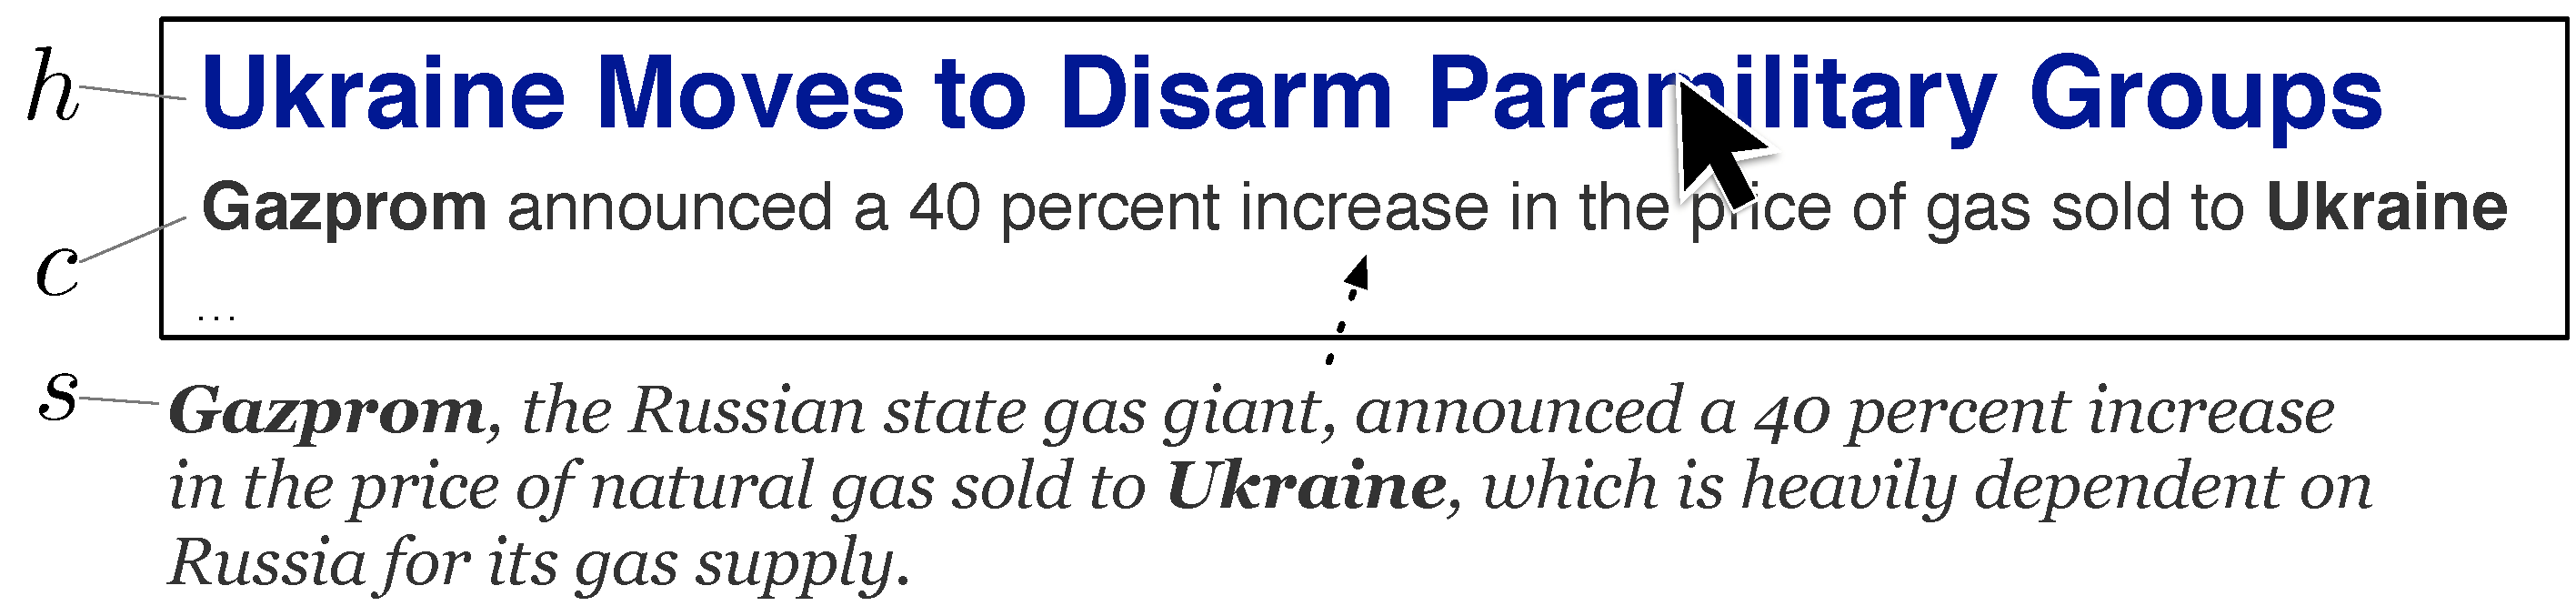
\includegraphics[width=9cm]{qf.pdf}
\caption{Search interfaces often require compressions with length and lexical constraints. In this case, the user has queried for ``Pemex contracts"; a system returns a related link and a short compression which contains the query terms}
\label{f:qf}
\end{figure}


\section{Compression and constraints}

In this work, we present a new method for compressing sentences, which leverages the predictive power of neural methods while accommodating lexical and length constraints. We compare our \textbf{transition-based} method to traditional \textbf{ILP-based techniques}, which also give a user such control and to baseline \textbf{LSTM taggers} which cannot accommodate such constraints.


\begin{table*}[htb!]
\begin{tabular}{cccc}
\textbf{Approach} & \textbf{Worst-case complexity} & \textbf{Constrained} & \textbf{Allows supervision} \\ \hline
LSTM taggers      & linear              & no     &    yes      \\   
linear programming              & exponential         & yes    &    yes   \\
transition-based (this work)       & quadratic*           & yes    &      yes   \\
\end{tabular}
\caption{\ahcomment{Blah blah blah blah}}
\end{table*}

\subsection{Constrained compression with ILPs}

One common approach for shortening sentences formulates compression as an integer linear programming (ILP) task. ILP-based methods assign binary variables to each token in a sentence or nested subtree in a dependency parse. These variables indicate if a word or subtree should be included in a compression. Each such sentence component is also assigned a local weight, indicating its worthiness for inclusion in a shortened sentence.\footnote{Local weights are either learned via structured perceptron techniques; or inferred from corpus statistics, tf-idf scores or language models.}

ILP methods represent the overall quality of a compression by summing the local weights of sentence components to compute a global objective score.  The problem of identifying the best possible solution fo an integer programming compression objective is exponential in the number of tokens or number of subtrees in the input, as each corresponding binary variable may be set to 0 or 1. Researchers use off-the-shelf ILP solvers to identify the highest-scoring compression, from among the exponential possible configurations of binary variables. ILP methods can be joined with structured-perceptron techniques to make use of supervised corpora of sentence--compression pairs \cite{filippova2013overcoming}.

This integer linear programming approach also easily accommodates constrained compression. When performing ILP-based compression, researchers will already customarily add constraint terms to the ILP objective in order to preserve the meaning of a sentence (e.g. don't remove negations) or to ensure that output forms a valid dependency tree (e.g. each subtree must have a parent vertex). Adding additional length or lexical requirements is trivial: practitioners must specify that optimal solutions must be shorter than some character budget and must specify that binary variables marking inclusion of particular words must be set to 1. 

\subsection{Transition-based constrained compression}

In this work, we present an alternative method for shortening sentences under lexical and length constraints. Our transition-based technique compresses a sentence over $M$ time steps, by adding and removing $M$ different subtrees from a dependency parse, one after another. This method recalls early solutions to the compression problem \cite{Jing2000SentenceRF,Knight2000StatisticsBasedS}, which also shortened sentences by executing grammatically-motivated operations on syntactic representations of trees. \ahcomment{argue for coverage w/ F and A at some point} We present the formal details in \S\ref{s:system}.

Like ILP-based methods, transition-based approaches can easily accommodate lexical and length restrictions. At a high-level, such methods need to add subtrees which contain query terms and remove subtrees which do not contain subtrees, until identifying a compression which satisfies the length constraints. In this work, we show that transition-based methods incur much smaller computational costs than integer programming techniques. We also show that transition-based methods achieve higher token-level F1 scores than ILP-based method on constrained compressions, by making use of large corpora of gold standard sentence--compression pairs.

\subsection{Unconstrained compression with LSTMs}

We contrast transition-based compression and integer programming approaches with LSTM taggers for the compression task \cite{filippova2015sentence}. Such taggers achieve state-of-the-art scores on extractive sentence compression, using sequence-to-sequence models that label tokens with a 1 or a 0 indicating if the token should be included in a summary. This encoder--decoder approach is linear in the token length of a the input sentence, and achieves a state-of-the art token-level F1 score. However, at this time, LSTM taggers are unsuitable for query-focused applications because such methods cannot enforce lexical or length requirements. This limitation might be examined in future research.

\section{Transition-based sentence compression}\label{s:system}

In this work, we define a neural, transition-based sentence compression system, inspired by recent successes in neural dependency parsing \cite{D14-1082}. Let ${(V_s,E_s)}$ denote the original, unchanging dependency parse of a sentence. At each timestep during compression, our system has a state ${(V_c,E_c)}$, which is some subgraph of ${(V_s,E_s)}$. The compression ${(V_c,E_c)}$ may or may not be fully-connected. 

We define two operations which modify the state. The operation \textsc{Prune}($v_c$), removes the subtree rooted at $v \in V_c$ from ${(V_c,E_c)}$. The operation \textsc{Insert}($v_s$), copies the subtree rooted at $v \in V_s$ in the original sentence and adds it to the compression ${(V_c,E_c)}$. After executing a sequence of $\textsc{Prune}$ and $\textsc{Insert}$ operations, all tokens in ${(V_c,E_c)}$ are linearized in their original order to return a shortened sentence. We initialize the state with an empty subgraph. 

We defined $\textsc{Prune}$ and $\textsc{Insert}$ via empirical experiment: we found that for all compressions in a large, standard  corpus \cite{filippova2013overcoming} there exists an oracle path of at most $|V_s|$ $\textsc{Prune}$ and $\textsc{Insert}$ operations which can fully reconstruct the shortened sentence. 

\begin{figure*}[htb!]
\centering
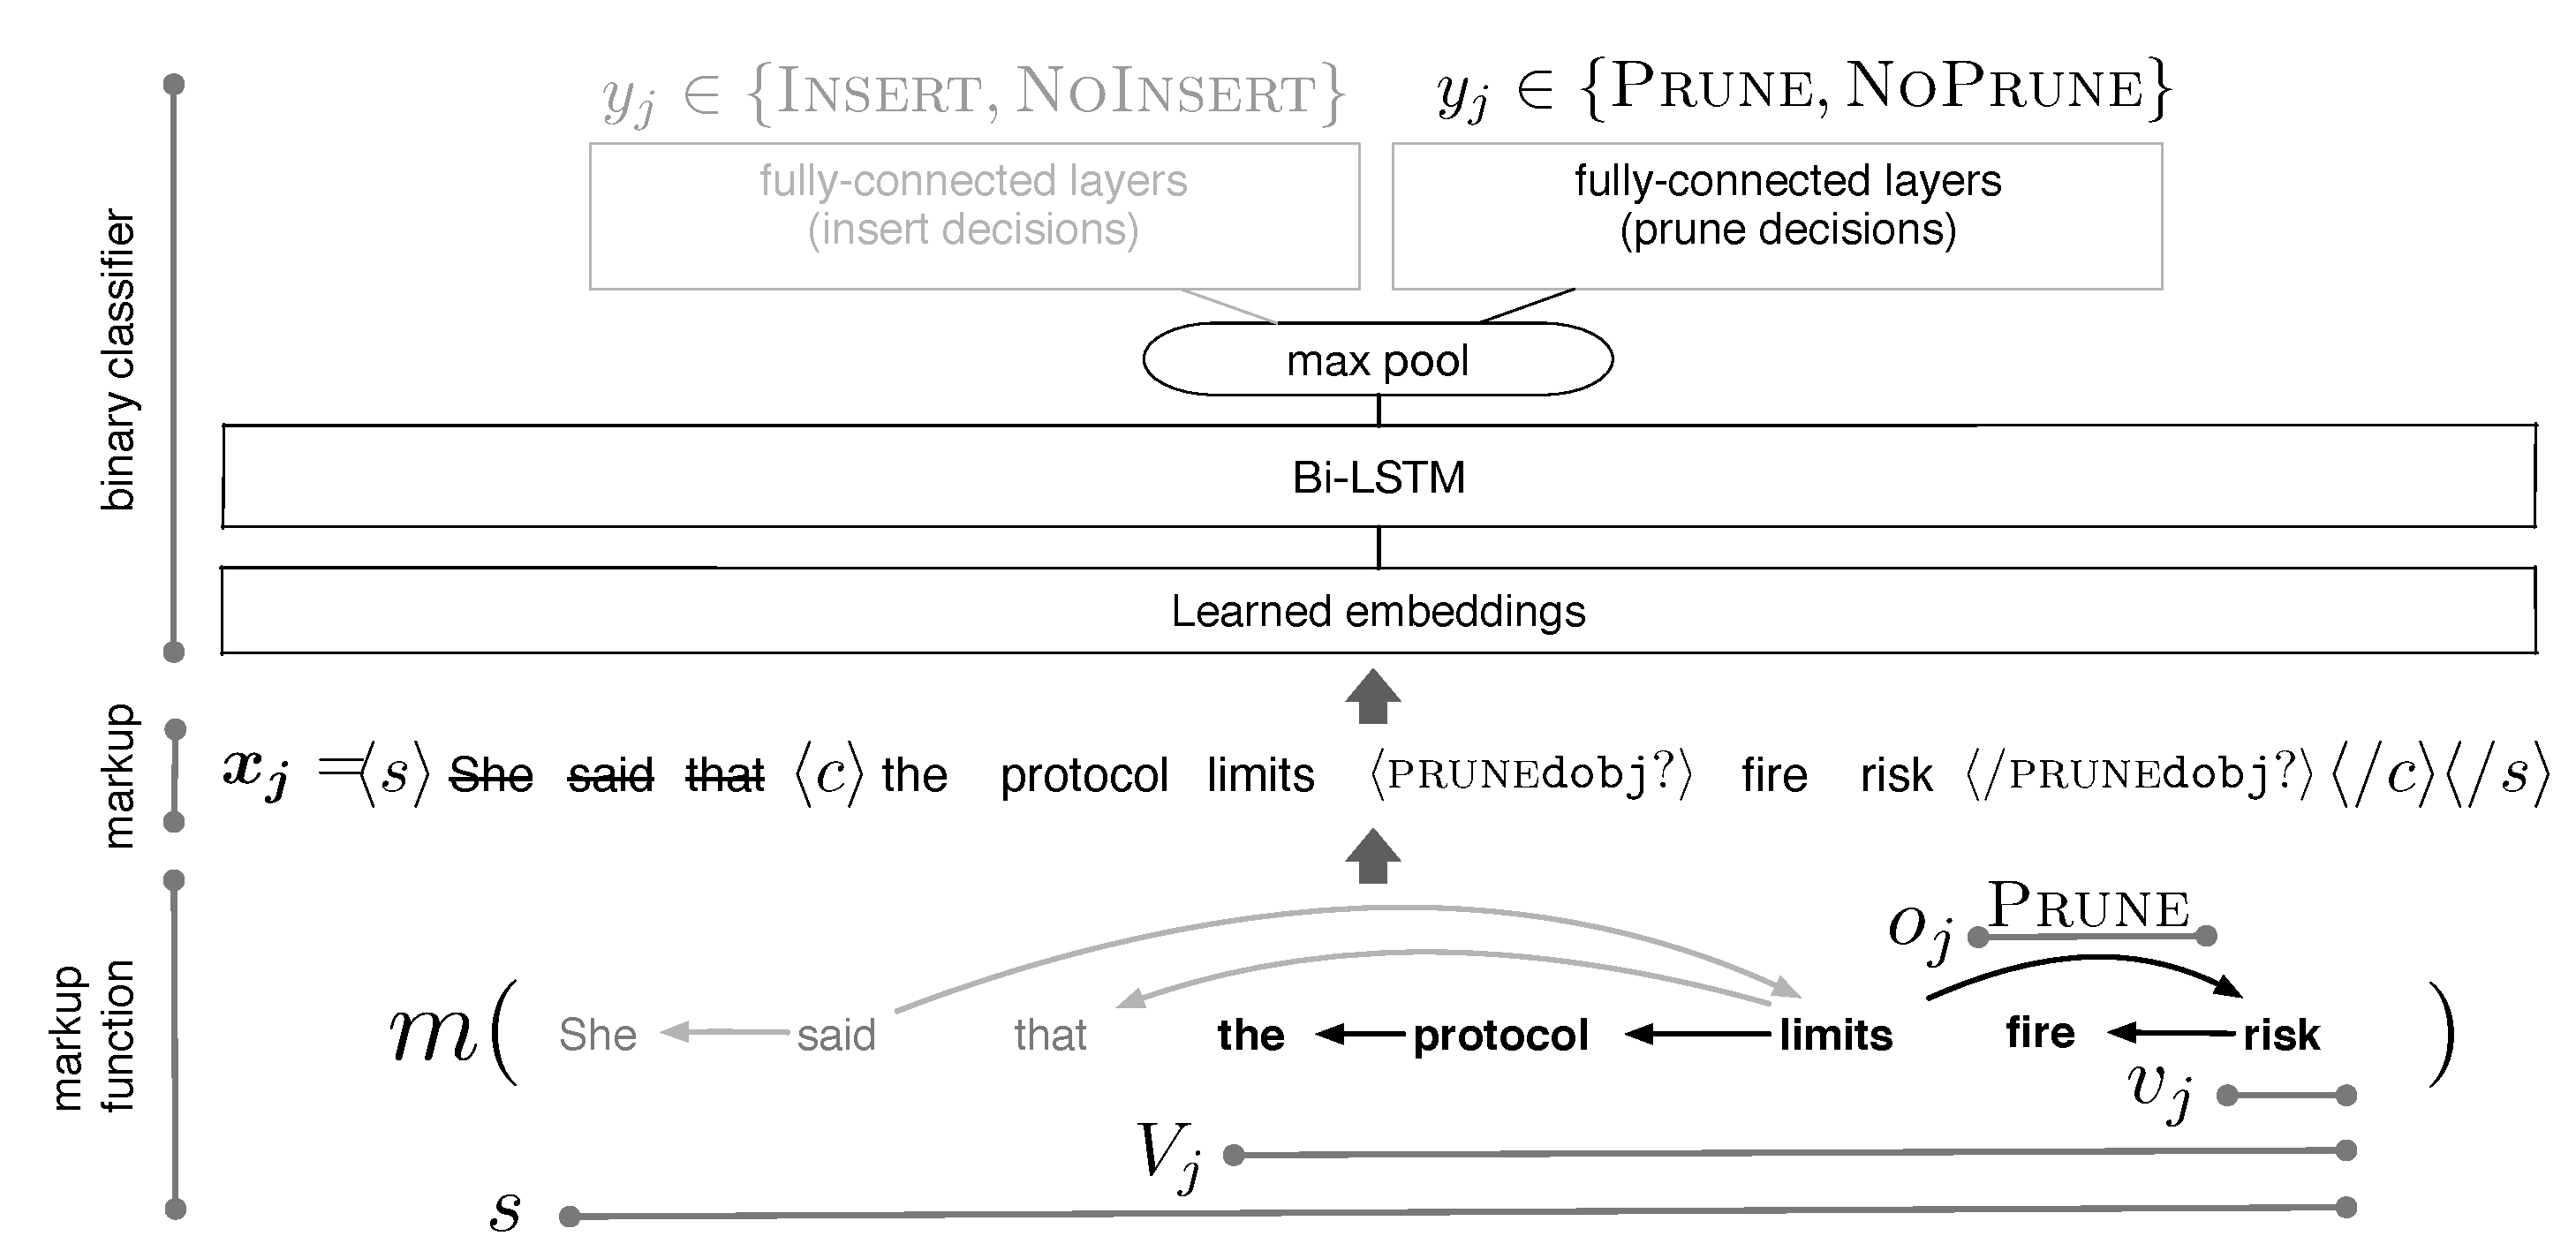
\includegraphics[width=.75\textwidth]{example.pdf}
\caption{\ahcomment{TODO}}
\label{f:example}
\end{figure*}

Like \cite{D14-1082}, we use a large supervised corpus to assign an oracle operation to each $v \in V_s$, by walking the dependency parse of an original sentence, breadth-first and identifying the oracle operation performed at each vertex. For roughly two thirds of vertexes in the breath-first walk, the oracle does not execute a $\textsc{Prune}$ or $\textsc{Insert}$ operation. In these cases, we say that the oracle executes a $\textsc{Nop}$, which leaves ${(V_c,E_c)}$ unmodified. 

In our transition-based compressor, we say that only some operations are valid for some configurations of the state. If some vertex $v \in V_s$ is also included in the compression, then we say that $\textsc{Insert}(v)$ is not valid as $v$ is already present in the compression. Similarly, if some vertex $v^{\prime} \notin V_c$ is not included in the compression, then we say that $\textsc{Prune}(v^{\prime})$ is not valid as $v^{\prime}$ cannot be pruned.

Because all $v \in V_s$ are either in $V_c$ or not in $V_c$, for any given vertex--state pair either the operation \textsc{Prune} is valid or the operation \textsc{Insert} is valid, but not both. We can therefore assign two subtypes of $\textsc{Nop}$ operation. If the oracle does not prune a given subtree, we say that the oracle executes $\textsc{Nop}_P$. If the oracle does not insert a given subtree, we say that the oracle executes $\textsc{Nop}_I$.

\section{Experiment 1: constrained compression}

We use a large, standard dataset of sentence--compression pairs from \citet{filippova2013overcoming} to both train and evaluate different approaches to length and lexically constrained compression. Using the dataset in this matter requires reinterpreting gold standard data, which does not specify either a query or length constraint. After re-tokenizing, parsing and tagging NER spans with Stanford CoreNLP \cite{corenlp}, we define all NER tokens which lie within the gold compression as the query, $q$.\footnote{We use a standard 3-class definition of NER; for our purposes, entities are people, locations or organizations.} Formally, $Q$ is a list of tokens. We also define the character length of the gold-standard compression as the maximum number of characters for the constrained compression. This interpretation allows us to redefined the corpus of sentence--compression pairs as a corpus of 4-tuples $(q,s,b,c)$, where $q$ is the query, $s$ is the original sentence, $b$ is the character budget and $c$ is some readable compression which satisfies the length and lexical constraints. We then use token-level F1, to measure how well an ILP-based method and a transition-based method method can reconstruct each known-good compression $c$, given $q,s$ and $b$. Token-level F1 is the standard automatic evaluation metric for the sentence compression task. \ahcomment{human eval}
    
\begin{table}[htb!]
\begin{tabular}{ll}
\centering
Approach & F1 \\ \hline
Human acceptability supervision         &  A          \\
F and A (2013)    & B           \\
C and L (2008)    & C        \\
Neural subtree deletion methods? &  D    \\   
\end{tabular}
\end{table}

\subsection{Implementation: ILP-based compression}

To our knowledge, there is no public code release for this model. We reimplement the method, and achieve similar token-level F1 scores. We use the Gurobi engine (v7) to solve the ILP. There are minor discrepancies between our implementation which have to do w/ different syntactic formalisms, different optimizers and our decision to re-parse and re-tokenize everything. We make note of some differences in the appendix. We also modify the method to accept (optional) query and budget constraints. 

\ahcomment{gurobi pool search mode is turned ON which makes everythign go slower. you should turn this off if you start making arguments about wall clock time}

\ahcomment{do you train the ILP to accept query terms? that is not really a baseline. }

\ahcomment{100k in training set. we do too }

\ahcomment{how to assess convergence}

\ahcomment{implementing get Q prefers to get the root. }


\ahcomment{what do they do in IR for query biased snippets? Hamed, John, Jieppu.
 (Prior study suggests that grammatical malformations cause readability errors in search results \cite{kanungo2009predicting}).}



\subsection{Implementation: transition-based compression}

Identifying oracle compressions defines a set of tuples: ${((V_c,E_c)_j, y_j)}$, where $(V_c,E_c)_j$ is the state of the system at step $j$ along the oracle path and $y_j \in  \{ \textsc{Prune}(v_c), \textsc{Insert}(v_s), \textsc{Nop}_P, \textsc{Nop}_I \}$ is the oracle operation at step $j$. We then train an ordinary LSTM classifier to predict the oracle operation, given the state. 

The input to our classifier is a sequence of embeddings which indicate how an operation would modify the current state. To create the sequence, we linearize all tokens in $V_c$ in their original order, and add out-of-vocabulary SOS and EOS symbols marking the beginning and end of the sequence. If the oracle operation is either $\textsc{Insert}$ or $\textsc{Nop}_I$, we also add the proposed additional tokens to the input sequence; again preserving original token order.

In addition, we also add out-of-vocabulary marker symbols at the beginning and end of the subsequence which would be removed or added by an $\textsc{Insert}$ or $\textsc{Prune}$. These marker symbols are formed by concatenating the type of the proposed operation (i.e. prune or insert) with the typed dependency governing the root of the subtree to be added or removed. Figure \ref{f:example} shows an example of a token sequence. Such marker symbols allow us to easily encode important aspects of the overall tree structure in a standard sequence classifier. 

During training, we look up each token in the sequence in an embeddings matrix and pass these embeddings to a Bi-LSTM. Following recent work on LSTM classification for sentence-level tasks \cite{D17-1070}, we use a max pooling layer to encode a variable-length sequence into a fixed-length vector, which we pass through a sigmoid and then softmax layer to predict the oracle operation. We train using cross entropy loss, weighting training examples in proportion to their prevalence in the dataset. \ahcomment{details here}

\ahcomment{comment on projectivity}
\ahcomment{details of embeddings}
\ahcomment{loss function}
\ahcomment{tuning}

We execute greedy, breadth first compression to reconstruct sentences. We walk original dependency parse, breadth-first and execute whichever valid operation is assigned the largest probability under the model. This achieves a token-level F1 score of \ahcomment{TODO}

\subsection{Preprocessing with extract}
Extract preprocessing. Make up a few simple rules. They will help a bunch. Only like 6 dependency types work at all for extract. This is in realfake/createdata/extract at the moment.



\ahcomment{How will we deal with semantics? Brendan email about subsective adjectives ellie pavlik work. }


\section{Computational experiments part 2: investigating properties of q,s,r compression}
\begin{enumerate}
\item{q = a list of 1 to 3 NER}
\item{r = random}
\item{What is the size of the minimum compression?}
\item{Reachability by budget by position of q in syntax tree. (If q is more than one entity then how the entities are dispersed across the tree probably matters a bunch too).}
\item{Hang on. reachability == min compression, eh? if min compression $>$ b, it is clearly bad.}
\item{Avoid computational waste w/ grammar.  Examine: ops you never have to worry about if you prune a branch v. dependency type deletion endorsement rate. Some ops get rid of lots of tokens w/ very high probability of deletion endorsements: e.g. parataxis (a great op!). By contrast: pruning a noun subj destroys acceptability and usually does not delete many tokens. Not worth the risk!}
\item{What is the empirical number of ops (i.e. decisions you have to make about pruning) if you greedily drop branches but never drop if the single op probability is less than $p$? My guess is you can make this problem way, way, simpler than implied by exponential formulation. Is it really quadratic?}
\item{Distribution of number of ops used for different q and r: when choosing ops at random? when choosing greedily? When pruning $\propto$ p(endorsement)?}
\item{Other stuff: min compression, reachability, operations saved w/ big prunes? position of query in the tree?}
\end{enumerate}

\section{computational experiments part 3: computational costs}

\ahcomment{this needs to be rewritten}

In the worst case, an iterative deletion method will prune one singleton subtree (consisting of only one vertex) at each of the $M$ timesteps during compression. (Starting from the leaves and proceeding to the root of the original dependency parse). If a dependency parse contains $V$ original vertexes, and each remaining vertex is evaluated for possible deletion at each timestep, then the iterative deletion method requires at most ${\sum_{i = 0}^M V - i = O(V^2)}$ operations.

This worst case represents the theoretical upper bound of iterative deletion approaches. In practice, there is a substantial gap between the mathematical properties of the iterative deletion algorithm and the linguistic properties of English syntax. Coherent english sentences require verbs and subjects. Coordinated English phrases must be joined with a conjunction. Prepositions cannot be removed from the start of an English prepositional phrase. In section \S\ahcomment{TODO} we examine how a dataset of human judgements of the well-formedness of shortened sentences can dramatically reduce the empirical complexity of the iterative deletion algorithm by blocking obviously terrible prunes. While in principle there are an exponential number of possible sentence compressions, in practice there is a much smaller set of fluid or coherent shortened sentences. 

In section \S\ahcomment{TODO} we also examine how the order of subtree deletion affects performance: intuitively, pruning large trees early in deletion removes the need to evaluate their many subtrees later in the deletion process.



\section{Related work}

Traditional study of sentence compression is closely aligned with text summarization techniques that select and  shorten sentences \cite{Knight2000StatisticsBasedS,vanderwende2007beyond,clarke2008global,Nenkova2012ASO}. 
In these settings, it is important for compressions to retain ``important'' information from source sentences because they must stand-in for longer sentences within summaries.

Our concern with lexical constraints is better suited to applications in which user queries define important information in documents. For instance, our length and lexically-constrained compressions could be used in information retrieval systems that summarize search results using query-based snippets on a search engine results page \cite{tombros1998advantages,Metzler2008MachineLS}. Often, such snippets must contain query terms. \ahcomment{screenshot?}

Our method could also be used for particular forms of query-focused summarization, such as summarizing people \cite{w04} or companies \cite{filippova2009company} which might require a hard lexical constraint. (Other work on query-focused summarization \cite{das} assumes softer constraints). 

Length and lexically constrained compressions could also be used as part of new forms of search user interfaces \cite{hearst2009search}, such as concept map browsers \cite{falke2017graphdocexplore}. Our interest in this problem arose from constructing one such novel search system.

\section{Conclusion}
\ahcomment{TODO}

\section{Appendix}

In this work, we reimplement the method of \citet{filippova2013overcoming}, who in turn implement transformations described in \citet{filippova2008dependency}. There are inevitable discrepancies between implementations. Some differences arise from differences in syntactic formalisms. Most importantly, prior work uses a tree transformation method which is no longer strictly compatible with UD. (For instance, the transformation assumes the PPs are headed by prepositions, which is not true in UD). Therefore, in implementing the ILP, we use the enhanced dependencies representation from CoreNLP \cite{Schuster2016EnhancedEU}. The augmented modifiers and augmented conjuncts in this representation create parses that are very similar to the transformed trees described in \citet{filippova2008dependency}. Prior also describes a syntactic constraint based on the \rdep{sc} relation, which is not included in UD. We therefore exclude this constraint.

Other differences between arise from diverging output from part-of-speech taggers. Prior work modifies a dependency tree by adding an edge between the root note and all verbs in a sentence, as a preprocessing step. This ensures that subclauses can be removed from parse trees to form compressions. However, we found that replicating this transform made it impossible for the ILP to create some gold compressions in the \citet{filippova2013overcoming} dataset; likely because different part-of-speech taggers disagree on some verb tags. We therefore add an edge between the root node and \textit{all} tokens in a sentence; we confirm that with this change the ILP can always output the gold compression.

Prior work does not specify all features in the structured perceptron model. We implement every feature discussed in the published work.

\ahcomment{Sort of hard to tell what formalism F and A use. I thnk it is stanford, but they don't come out and say it.They cite Nivre's book which references the malt parser which seems to use stanford deps. but I don't see mention of the ``in" relation referenced in F and A paper in a guide to stanford deps. Writing around it.}

\bibliography{abe}
\bibliographystyle{acl_natbib}

\end{document}
